\documentclass[tikz,border=2mm]{standalone}
\usepackage{tikz}
\usepackage{xcolor}
\usetikzlibrary{positioning, arrows.meta}
\usetikzlibrary{shapes.geometric, arrows,fit}
\usetikzlibrary{shapes.multipart}
\definecolor{gray}{rgb}{0.44, 0.5, 0.56}
\definecolor{egyptianblue}{rgb}{0.06, 0.2, 0.65}
\definecolor{spanishviolet}{rgb}{0.25,0.18,0.53}
\definecolor{byzantium}{rgb}{0.45,0.17,0.42}
\definecolor{amaranthpurple}{rgb}{0.64,0.15,0.29}
\definecolor{amaranthred}{rgb}{0.83, 0.13, 0.18}
\definecolor{dcp}{rgb}{0.96,0.18,0.18}


\tikzstyle{node}=[thick,circle,minimum size=12,draw=egyptianblue]
\tikzstyle{emb} =[rectangle, thick,
text centered, 
minimum width=0.3cm, 
minimum height=0.2cm,
draw=black]

\begin{document}

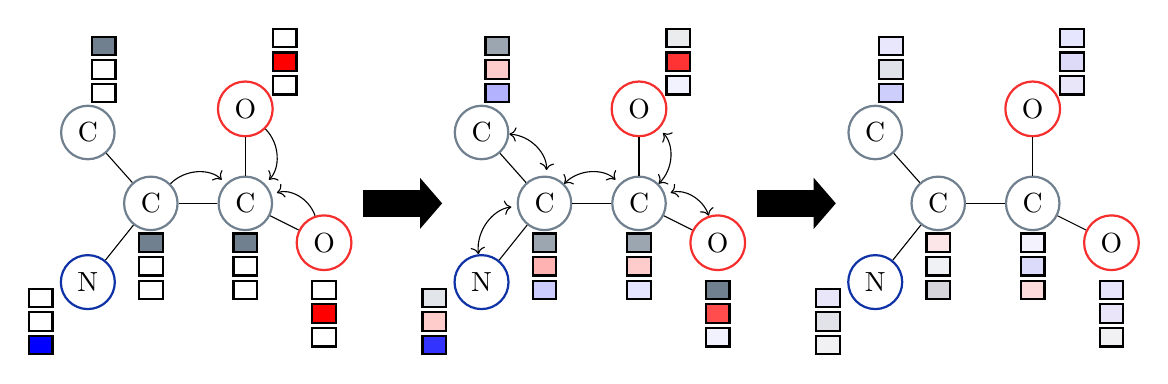
\begin{tikzpicture}[squa/.style={
  draw,
  inner sep=4pt,
  font=\Large,
}]
\tikzset{every node/.style={rectangle split, draw, minimum width=.5cm}}

\node [style=node,draw=gray] (0) at (0, 0) {C};
\node [style=node,draw=dcp] (1) at (0, 1.20) {O};
\node [style=node,draw=dcp] (2) at (1, -0.5) {O};
\node [style=node,draw=gray] (3) at (-1.2,0) {C};
\node [style=node,draw=gray] (4) at (-2.0,0.9) {C};
\node [style=node] (5) at (-2.0,-1.0) {N};

\node[emb,fill=gray] (0a) at (0,-0.5) {};
\node[emb] (0b) at (0,-0.8) {};
\node[emb] (0c) at (0,-1.1) {};

\node[emb] (1a) at (0.5,1.5) {};
\node[emb,fill=red] (1b) at (0.5,1.8) {};
\node[emb] (1c) at (0.5,2.1) {};

\node[emb] (2a) at (1,-1.1) {};
\node[emb,fill=red] (2b) at (1,-1.4) {};
\node[emb] (2c) at (1,-1.7) {};

\node[emb,fill=gray] (3a) at (-1.2,-0.5) {};
\node[emb] (3b) at (-1.2,-0.8) {};
\node[emb] (3c) at (-1.2,-1.1) {};

\node[emb,fill=gray] (4a) at (-1.8,2.0) {};
\node[emb] (4b) at (-1.8,1.7) {};
\node[emb] (4c) at (-1.8,1.4) {};

\node[emb](5a) at (-2.6,-1.2){};
\node[emb](5a) at (-2.6,-1.5){};
\node[emb,fill=blue](5a) at (-2.6,-1.8){};

\draw (0) to (1);
\draw (0) to (2);
\draw (0) to (3);
\draw (3) to (4);
\draw (3) to (5);

\draw [-{>[sep=2pt]}] (1) to [bend left=45] (0);
\draw [-{>[sep=2pt]}] (2) to [bend right=45] (0);
\draw [-{>[sep=2pt]}] (3) to [bend left=45] (0);

\draw[-{Triangle[width=18pt,length=8pt]}, line width=10pt](1.5,0) -- (2.5, 0);


\node [style=node,draw=gray] (0i) at (5, 0) {C};
\node [style=node,draw=dcp] (1i) at (5, 1.20) {O};
\node [style=node,draw=dcp] (2i) at (6, -0.5) {O};
\node [style=node,draw=gray] (3i) at (3.8,0) {C};
\node [style=node,draw=gray] (4i) at (3.0,0.9) {C};
\node [style=node] (5i) at (3.0,-1.0) {N};

\node[emb,fill=gray!70] (0ia) at (5,-0.5) {};
\node[emb,fill=red!20] (0ib) at (5,-0.8) {};
\node[emb,fill=blue!10] (0ic) at (5,-1.1) {};

\node[emb,fill=blue!5] (1ia) at (5.5,1.5) {};
\node[emb,fill=red!80] (1ib) at (5.5,1.8) {};
\node[emb,fill=gray!15] (1ic) at (5.5,2.1) {};

\node[emb,fill=gray=!25] (2ia) at (6,-1.1) {};
\node[emb,fill=red!70] (2ib) at (6,-1.4) {};
\node[emb,fill=blue!5] (2ic) at (6,-1.7) {};

\node[emb,fill=gray!70] (3ia) at (3.8,-0.5) {};
\node[emb,fill=red!30] (3ib) at (3.8,-0.8) {};
\node[emb,fill=blue!20] (3ic) at (3.8,-1.1) {};

\node[emb,fill=gray!70] (4ia) at (5-1.8,2.0) {};
\node[emb,fill=red!20] (4ib) at (5-1.8,1.7) {};
\node[emb,fill=blue!30] (4ic) at (5-1.8,1.4) {};

\node[emb,fill=gray!20](5ia) at (5-2.6,-1.2){};
\node[emb,fill=red!20](5ia) at (5-2.6,-1.5){};
\node[emb,fill=blue!80](5ia) at (5-2.6,-1.8){};

\draw (0i) to (1i);
\draw (0i) to (2i);
\draw (0i) to (3i);
\draw (3i) to (4i);
\draw (3i) to (5i);

\draw [<-{>[sep=2pt]}] (4i) to [bend left=45] (3i);
\draw [<-{>[sep=2pt]}] (5i) to [bend left=45] (3i);
\draw [<-{>[sep=2pt]}] (3i) to [bend left=45] (0i);
\draw [<-{>[sep=2pt]}] (0i) to [bend right=45] (1i);
\draw [<-{>[sep=2pt]}] (2i) to [bend right=45] (0i);

\draw[-{Triangle[width=18pt,length=8pt]}, line width=10pt](6.5,0) -- (7.5, 0);


%%%%%%%%%%%%%%%%%%%%%%%%%%%

\node [style=node,draw=gray] (0ii) at (10, 0) {C};
\node [style=node,draw=dcp] (1ii) at (10, 1.20) {O};
\node [style=node,draw=dcp] (2ii) at (11, -0.5) {O};
\node [style=node,draw=gray] (3ii) at (8.8,0) {C};
\node [style=node,draw=gray] (4ii) at (8.0,0.9) {C};
\node [style=node] (5ii) at (8.0,-1.0) {N};

\node[emb,fill=gray!40!red!20!blue!5] (0iia) at (10,-0.5) {};
\node[emb,fill=red!30!gray!20!blue!15] (0iib) at (10,-0.8) {};
\node[emb,fill=blue!20!gray!10!red!15] (0iic) at (10,-1.1) {};

\node[emb,fill=gray!20!red!20!blue!10] (1iia) at (10.5,1.5) {};
\node[emb,fill=red!50!gray!20!blue!15] (1b) at (10.5,1.8) {};
\node[emb,fill=blue!20!gray!10!blue!10] (1iic) at (10.5,2.1) {};

\node[emb,fill=gray!25!red!15!blue!10] (2iia) at (11,-1.1) {};
\node[emb,fill=red!50!red!20!blue!10] (2iib) at (11,-1.4) {};
\node[emb,fill=blue!30!red!10!gray!10] (2iic) at (11,-1.7) {};

\node[emb,fill=gray!40!blue!10!red!10] (3iia) at (10-1.2,-0.5) {};
\node[emb,fill=red!20!blue!10!gray!10] (3iib) at (10-1.2,-0.8) {};
\node[emb,fill=blue!30!red!10!gray!30] (3iic) at (10-1.2,-1.1) {};

\node[emb,fill=gray!40!red!20!blue!10] (4iia) at (10-1.8,2.0) {};
\node[emb,fill=red!20!blue!10!gray!20] (4iib) at (10-1.8,1.7) {};
\node[emb,fill=blue!10!gray!10!blue!20] (4iic) at (10-1.8,1.4) {};

\node[emb,fill=gray!20!red!20!blue!10](5iia) at (10-2.6,-1.2){};
\node[emb,fill=red!30!blue!10!gray!20](5iia) at (10-2.6,-1.5){};
\node[emb,fill=blue!60!red!10!gray!10](5iia) at (10-2.6,-1.8){};

\draw (0ii) to (1ii);
\draw (0ii) to (2ii);
\draw (0ii) to (3ii);
\draw (3ii) to (4ii);
\draw (3ii) to (5ii);


\end{tikzpicture}



\end{document}
